\documentclass[aspectratio=169]{beamer}
\usetheme[numbering=fraction]{metropolis}

% ── Ruban titre ───────────────────────────────────────────────
\makeatletter
\setlength{\metropolis@frametitle@padding}{1ex}
\makeatother

% ── Suppression des slides de transition de section ──────────
\metroset{sectionpage=none}

\usepackage[french]{babel}
\usepackage[T1]{fontenc}
\usepackage[utf8]{inputenc}
\usepackage{lmodern}
\usepackage{csquotes}
\usepackage{xcolor}
\usepackage{graphicx}
\usepackage{booktabs}
\usepackage{caption}
\usepackage{tikz}
\usetikzlibrary{arrows.meta,positioning,calc,decorations.pathmorphing}
\usepackage{varwidth}
\usepackage{colortbl}
\usepackage{array}
\usepackage{amsmath}
\usepackage{appendixnumberbeamer}
\graphicspath{{../../../results/figures/}{../../../results/morvan/figures/}{../../../results/sechilienne/figures/}{./}}

% ================================================================
% COULEURS
% ================================================================
\definecolor{myblue}{HTML}{1F4E79}
\definecolor{myblue2}{HTML}{2E6BA8}
\definecolor{myorange}{HTML}{E07B39}
\definecolor{mygreen}{HTML}{2E7D32}
\definecolor{myred}{HTML}{C0392B}
\definecolor{myteal}{HTML}{006064}
\definecolor{mylgray}{HTML}{F4F6F9}
\definecolor{mymgray}{HTML}{D0D8E4}
\definecolor{mydgray}{HTML}{4A5568}
% bandes radar (mêmes couleurs que les figures)
\definecolor{Lband}{HTML}{2E7D32}
\definecolor{Cband}{HTML}{7B4FA8}
\definecolor{cut}{HTML}{C0392B}
\definecolor{ctrl}{HTML}{1F77B4}

% ================================================================
% COULEURS BEAMER
% ================================================================
\setbeamercolor{frametitle}{bg=myblue, fg=white}
\setbeamercolor{progress bar}{fg=myblue, bg=gray!20}
\setbeamercolor{block title}{bg=myblue, fg=white}
\setbeamercolor{block body}{bg=mylgray}
\setbeamercolor{block title alerted}{bg=myorange, fg=white}
\setbeamercolor{block body alerted}{bg=mylgray}
\setbeamercolor{block title example}{bg=mygreen, fg=white}
\setbeamercolor{block body example}{bg=mylgray}
\setbeamercolor{alerted text}{fg=myorange}
\setbeamercolor{bibliography entry author}{fg=myblue}
\setbeamercolor{bibliography entry title}{fg=myblue}

\captionsetup{labelfont=bf, font=small}

\newcommand{\Lb}[1]{\textcolor{Lband}{\textbf{#1}}}
\newcommand{\Cb}[1]{\textcolor{Cband}{\textbf{#1}}}

% ================================================================
% COMMANDE SOUS-TITRE DE SLIDE
% ================================================================
\newcommand{\slidesubtitle}[1]{%
	\textcolor{myblue}{\small\textbf{#1}}%
	\par\vspace{3pt}%
}
% chiffre clé : couleur, valeur, légende
\newcommand{\keynum}[3]{%
	\begin{minipage}[t]{0.31\linewidth}\centering
		\textcolor{#1}{\Large\textbf{#2}}\\[1pt]
		\scriptsize #3
	\end{minipage}}

% ================================================================
% BIBLIOGRAPHIE
% ================================================================
\usepackage[backend=biber, style=authoryear,
maxcitenames=2, mincitenames=1,
isbn=false, eprint=false, doi=false, url=false]{biblatex}
\addbibresource{../../latex/references.bib}

\AtBeginDocument{%
	\renewcommand*{\mkbibnamefamily}[1]{\textnormal{#1}}%
	\renewcommand*{\mkbibnamegiven}[1]{\textnormal{#1}}%
	\renewcommand*{\mkbibnameprefix}[1]{\textnormal{#1}}%
	\renewcommand*{\mkbibnamesuffix}[1]{\textnormal{#1}}%
}
\DeclareCiteCommand{\parencite}
{\usebibmacro{prenote}}
{\textcolor{black}{(}\textcolor{myred}{\usebibmacro{cite}}\textcolor{black}{)}}
{\multicitedelim}
{\usebibmacro{postnote}}

% ================================================================
% PIED DE PAGE
% ================================================================
\setbeamercolor{footline}{bg=white, fg=black}
\setbeamerfont{footline}{size=\scriptsize}
\setbeamertemplate{footline}{%
	\hbox{%
		\begin{beamercolorbox}[wd=\paperwidth, ht=1.5ex,
			dp=0.6ex, leftskip=0.4cm,
			rightskip=0.4cm]{footline}
			\color{black}\rule{\paperwidth}{0.3pt}\par
			\vspace{-0.25em}
			\hfill \insertframenumber/\inserttotalframenumber
		\end{beamercolorbox}%
	}%
}

% ================================================================
% PAGE DE TITRE PERSONNALISEE
% ================================================================
\setbeamertemplate{title page}{%
	\begin{tikzpicture}[overlay, remember picture]
		\node[anchor=north west, xshift=0.5cm, yshift=-0.45cm]
		at (current page.north west)
		{
\includegraphics[height=0.9cm]{../../presentation/logos/logo_icube.png}};
		\node[anchor=north east, xshift=-0.5cm, yshift=-0.35cm]
		at (current page.north east)
		{
\includegraphics[height=1.3cm]{../../presentation/logos/logo_sertit.png}};
	\end{tikzpicture}%
	\vspace*{1.1cm}
	\vfill
	\begin{center}
		\footnotesize\textcolor{mydgray}{%
			Dossier de candidature -- Stage SERTIT / ICube (Université de Strasbourg)}

		\vspace{0.3em}
		\scriptsize\textcolor{mydgray}{%
			\og Exploration des bandes L et P (NISAR, BIOMASS) pour la détection de la déforestation
			et des glissements de terrain \fg}

		\vspace{0.9em}

		\begin{varwidth}{0.92\linewidth}
			\centering
			{\usebeamerfont{title}\usebeamercolor[fg]{title}%
				\inserttitle\par}
		\end{varwidth}

		\vspace{0.6cm}

		{\usebeamerfont{author}\usebeamercolor[fg]{author}%
			\insertauthor\par}

		\vspace{0.4cm}

		{\usebeamerfont{date}\usebeamercolor[fg]{date}%
			\insertdate\par}
	\end{center}
	\vfill
}

\title{\large
	Bande L (NISAR) contre bande C (Sentinel-1)\\
	sous forêt : coupes rases et glissement de terrain\\[4pt]
	{\normalsize Trois tests de faisabilité menés en amont du stage}
}
\author{%
	Candidat : \textbf{Mamadou G. Diallo}
}
\date{Novembre 2026}

% ================================================================
\begin{document}

\begin{frame}
	\titlepage
\end{frame}

% ================================================================
\section{Démarche}
% ================================================================

\begin{frame}{\phantom{x}}
	\frametitle{Pourquoi ce travail}
	\vspace{-6pt}\scriptsize
	\begin{columns}[T]
		\column{0.55\textwidth}
		\begin{block}{Contexte}
			\scriptsize
			\begin{itemize}
				\setlength{\itemsep}{2pt}
				\item \Lb{NISAR} (NASA-ISRO) fournit depuis 2025 une \Lb{bande L} gratuite et systématique sur
				l'Europe \parencite{kellogg2020nisar} ; produits de niveau~2 générés par \textbf{ISCE3}
				\parencite{isce3}.
				\item \textbf{ROSE-L} (Copernicus, vers 2028) prendra le relais en Europe \parencite{esa2020rosel}.
				\item \textbf{BIOMASS} (bande P) n'acquiert pas sur l'Europe de l'Ouest : perspective
				\parencite{quegan2019biomass}.
			\end{itemize}
		\end{block}
		\begin{block}{Question commune aux trois tests}
			\scriptsize
			Sous la forêt, la \Lb{bande L} (24~cm) garde-t-elle un signal exploitable là où la \Cb{bande C}
			(5,6~cm) le perd, pour détecter une \textbf{coupe} et pour suivre un \textbf{versant instable} ?
		\end{block}
		\column{0.42\textwidth}
		\begin{block}{Trois sites, une chaîne}
			\scriptsize
			\begin{enumerate}
				\setlength{\itemsep}{3pt}
				\item \textbf{Vosges} : une coupe rase datée (2,4~ha), trois géométries NISAR
				\item \textbf{Morvan} : 7 coupes, méthode du guide de l'Irstea transposée au radar, géométrie égale
				dans les deux directions
				\item \textbf{Séchilienne} : glissement boisé, phase interférométrique L contre C
			\end{enumerate}
			\vspace{2pt}
			Paquet Python réutilisable (\texttt{nisar\_s1}), graphes SNAP, configuration par site :
			transposable à ROSE-L.
		\end{block}
	\end{columns}
\end{frame}

\begin{frame}{\phantom{x}}
	\frametitle{Physique attendue}
	\begin{columns}[c]
		\column{0.50\textwidth}
		\centering
		\begin{tikzpicture}[scale=0.82]
			\fill[brown!30] (0,0) rectangle (8,0.3);
			\foreach \x in {0.8,2.3,3.8} {
				\fill[brown!70!black] (\x-0.08,0.3) rectangle (\x+0.08,2.4);
				\fill[green!50!black,opacity=0.75] (\x,2.9) ellipse (0.65 and 0.9);
			}
			\foreach \x in {5.2,6.1,7.0} { \fill[brown!60!black] (\x-0.15,0.3) rectangle (\x+0.15,0.45); }
			\node[font=\scriptsize] at (6.1,0.75) {coupe : sol nu, rémanents};
			\draw[-{Latex},very thick,Cband,decorate,decoration={snake,amplitude=1.2pt,segment length=4pt}]
			(1.0,5.2) -- (2.2,3.4);
			\node[Cband,font=\scriptsize\bfseries] at (0.7,5.45) {C, 5,6 cm};
			\node[Cband,font=\scriptsize,align=right,anchor=east] at (1.45,3.9) {s'arrête\\au feuillage};
			\draw[-{Latex},very thick,Lband,decorate,decoration={snake,amplitude=2.2pt,segment length=9pt}]
			(2.9,5.2) -- (3.75,1.2);
			\node[Lband,font=\scriptsize\bfseries] at (3.4,5.45) {L, 24 cm};
			\node[Lband,font=\scriptsize,align=left,anchor=west] at (4.55,2.0) {atteint troncs\\et sol};
		\end{tikzpicture}
		\column{0.48\textwidth}
		\begin{block}{Conséquences attendues}
			\footnotesize
			\begin{itemize}
				\setlength{\itemsep}{3pt}
				\item Feuilles mobiles, troncs stables : la forêt reste \textbf{cohérente} à 12~jours en
				\Lb{L}, pas en \Cb{C} \parencite{zebker1992decorrelation}
				\item Une coupe devient alors un \textbf{événement} net en cohérence \Lb{L}
				\item Sous un versant boisé, seule une phase cohérente permet de mesurer un
				\textbf{déplacement}
			\end{itemize}
		\end{block}
		\scriptsize\textcolor{mydgray}{Hypothèses fixées avant les calculs, puis testées site par site.}
	\end{columns}
\end{frame}

% ================================================================
\section{Coupes rases}
% ================================================================

\begin{frame}{\phantom{x}}
	\frametitle{Coupes rases (1/3) : Vosges, une coupe datée}
	\vspace{-6pt}
	\centering
	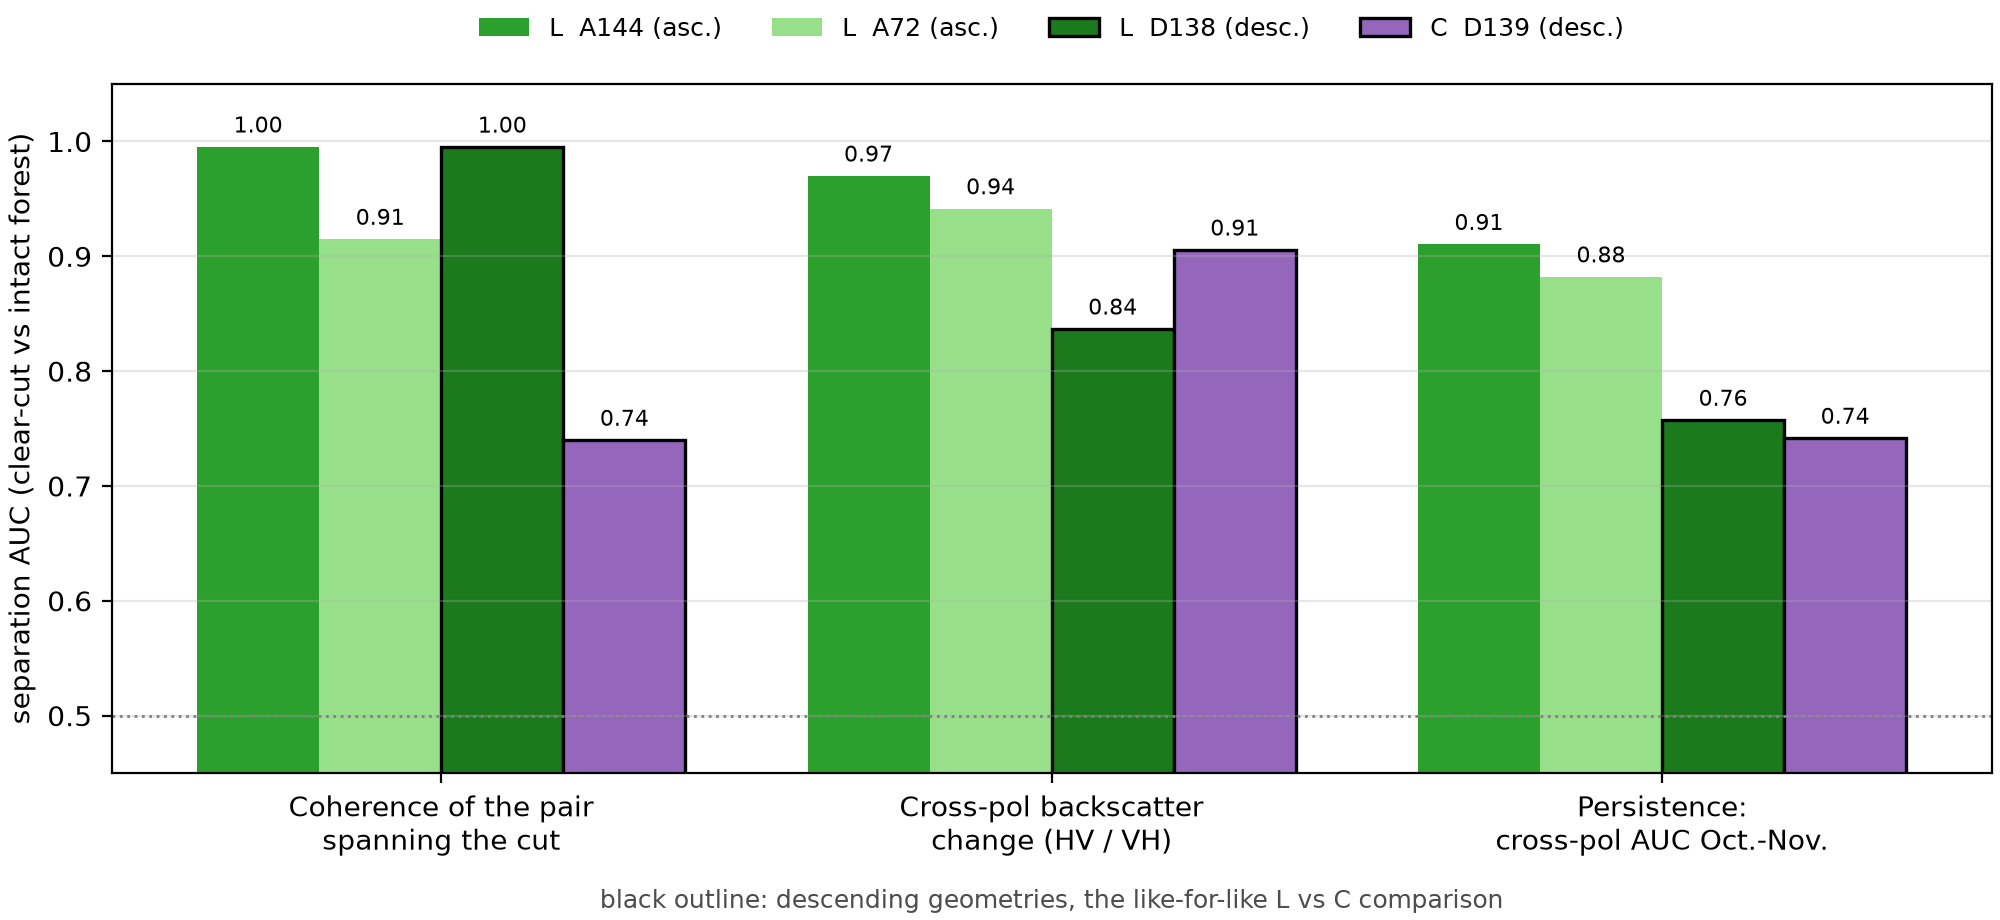
\includegraphics[width=0.74\linewidth, height=0.50\textheight, keepaspectratio]{summary_L_vs_C.png}

	\vspace{2pt}
	\keynum{Lband}{0,995}{AUC cohérence \Lb{L}\\paire encadrant la coupe}\hfill
	\keynum{Cband}{0,71--0,74}{AUC cohérence \Cb{C}\\mêmes dates}\hfill
	\keynum{myblue}{0,64--0,70}{cohérence \Lb{L} à 12~j\\de la forêt intacte (\Cb{C} : 0,28)}

	\vspace{4pt}
	\scriptsize\raggedright
	Coupe de 2,36~ha (août 2026), datée par Sentinel-2. L'avantage \Lb{L} est \textbf{interférométrique} dans
	les trois géométries ; en rétrodiffusion il dépend de la géométrie.
\end{frame}

\begin{frame}{\phantom{x}}
	\frametitle{Coupes rases (2/3) : Morvan, réplication selon le guide de l'Irstea}
	\vspace{-6pt}
	\centering
	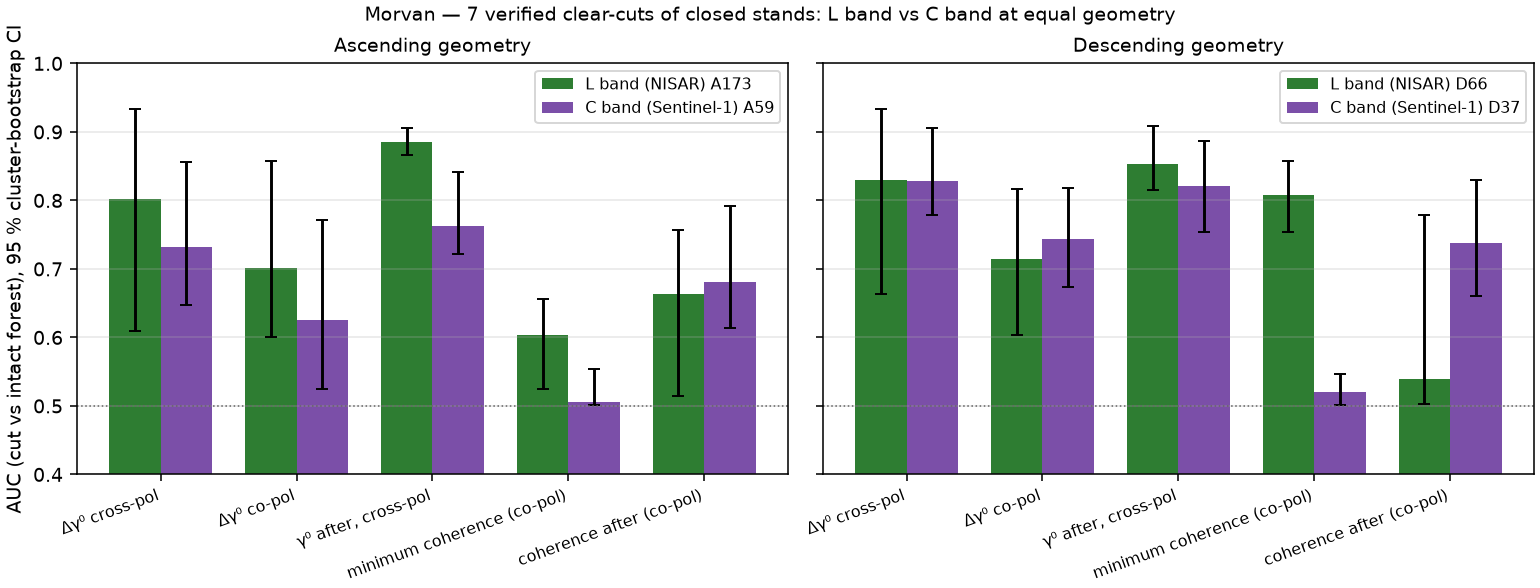
\includegraphics[width=0.80\linewidth, height=0.48\textheight, keepaspectratio]{m8_summary_L_vs_C.png}

	\vspace{2pt}
	\scriptsize\raggedright
	\begin{itemize}
		\setlength{\itemsep}{0pt}
		\item 7 coupes photo-interprétées (15~ha) ; géométrie égale : \Lb{L A173} / \Cb{C A59}, \Lb{L D66} / \Cb{C D37}
		\item Forêt intacte à 12~j : \Lb{0,35--0,71} contre \Cb{0,25--0,36} (plancher de l'estimateur) : H1 confirmée
		\item AUC de cohérence en descendante : \Lb{0,81} contre \Cb{0,52} ; rétrodiffusion croisée : AUC proches,
		contraste plus fort en \Lb{L}
	\end{itemize}
\end{frame}

\begin{frame}{\phantom{x}}
	\frametitle{Coupes rases (3/3) : la méthode du guide appliquée au radar}
	\vspace{-6pt}
	\centering
	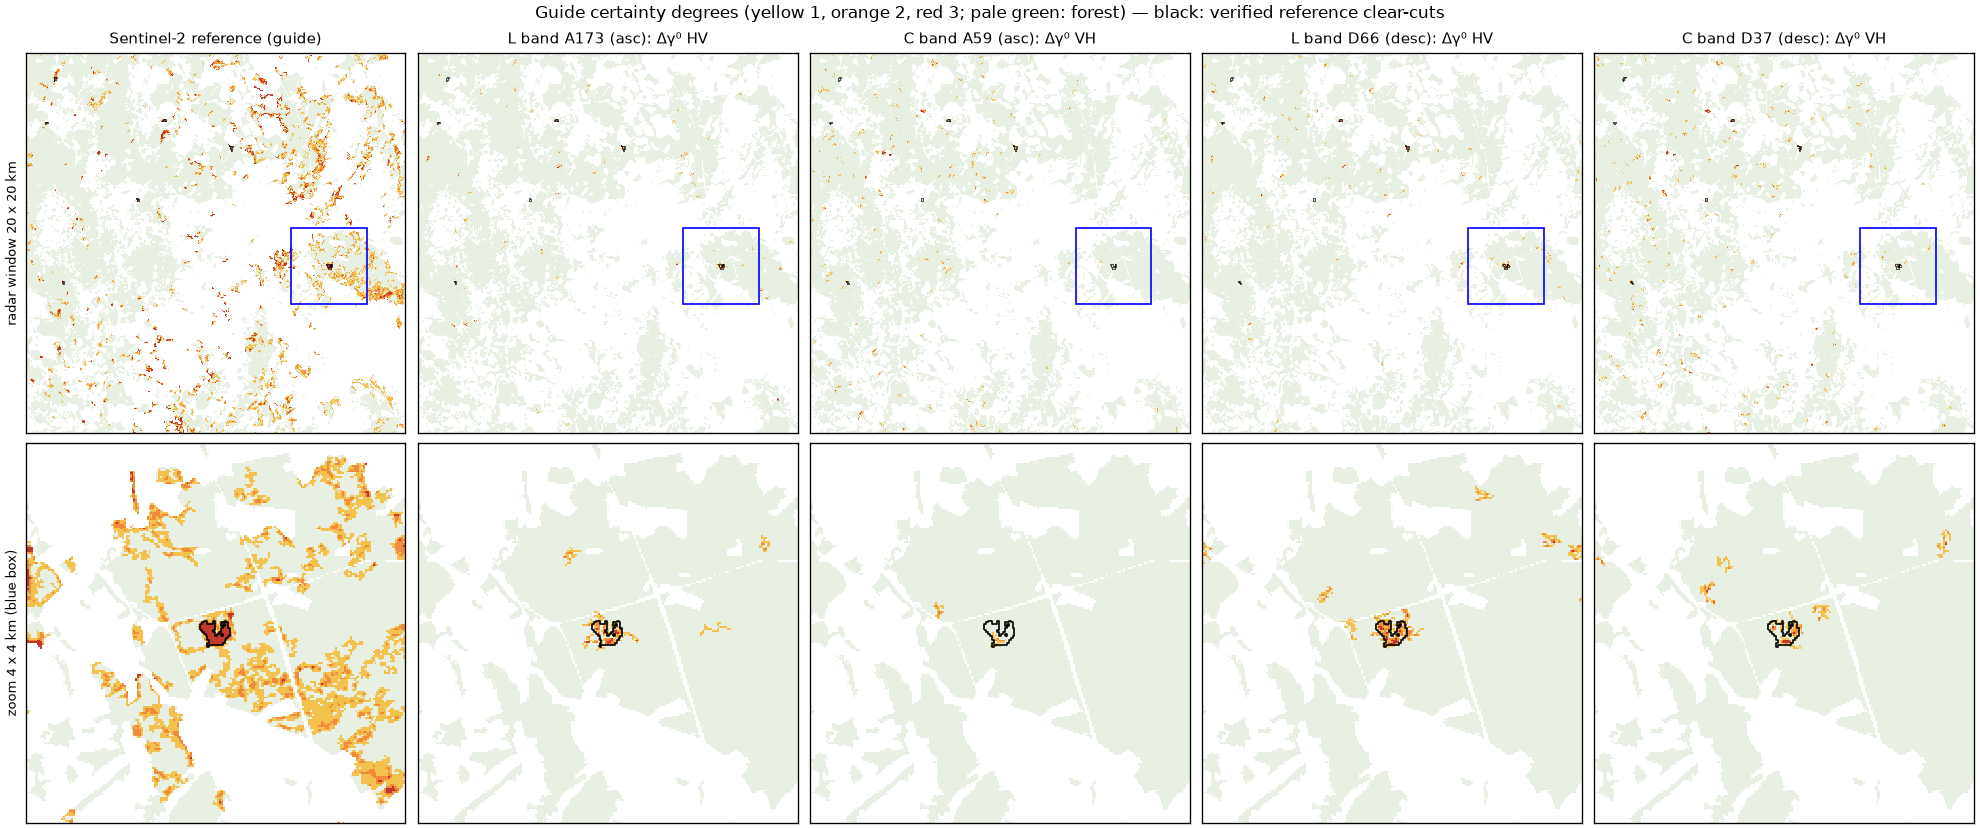
\includegraphics[width=\linewidth, height=0.46\textheight, keepaspectratio]{m6_guide_maps.png}

	\vspace{2pt}
	\keynum{Lband}{0,41}{kappa \Lb{L}\\5 coupes sur 7}\hfill
	\keynum{Cband}{0,08--0,16}{kappa \Cb{C}\\2 à 3 coupes sur 7}\hfill
	\keynum{myblue}{8,7~\%}{forêt signalée par le guide\\sur Sentinel-2 intra-saison}

	\vspace{4pt}
	\scriptsize\raggedright
	Seuils statistiques du guide ($m - k\sigma$), tamisage à 1~ha, matrice de confusion en surface. Le guide n'atteint
	pas son objectif de 10~\% d'erreur ici : la qualité de la référence domine tout.
\end{frame}

% ================================================================
\section{Glissement de terrain}
% ================================================================

\begin{frame}{\phantom{x}}
	\frametitle{Glissement (1/2) : Séchilienne, la phase sous la forêt}
	\vspace{-6pt}
	\centering
	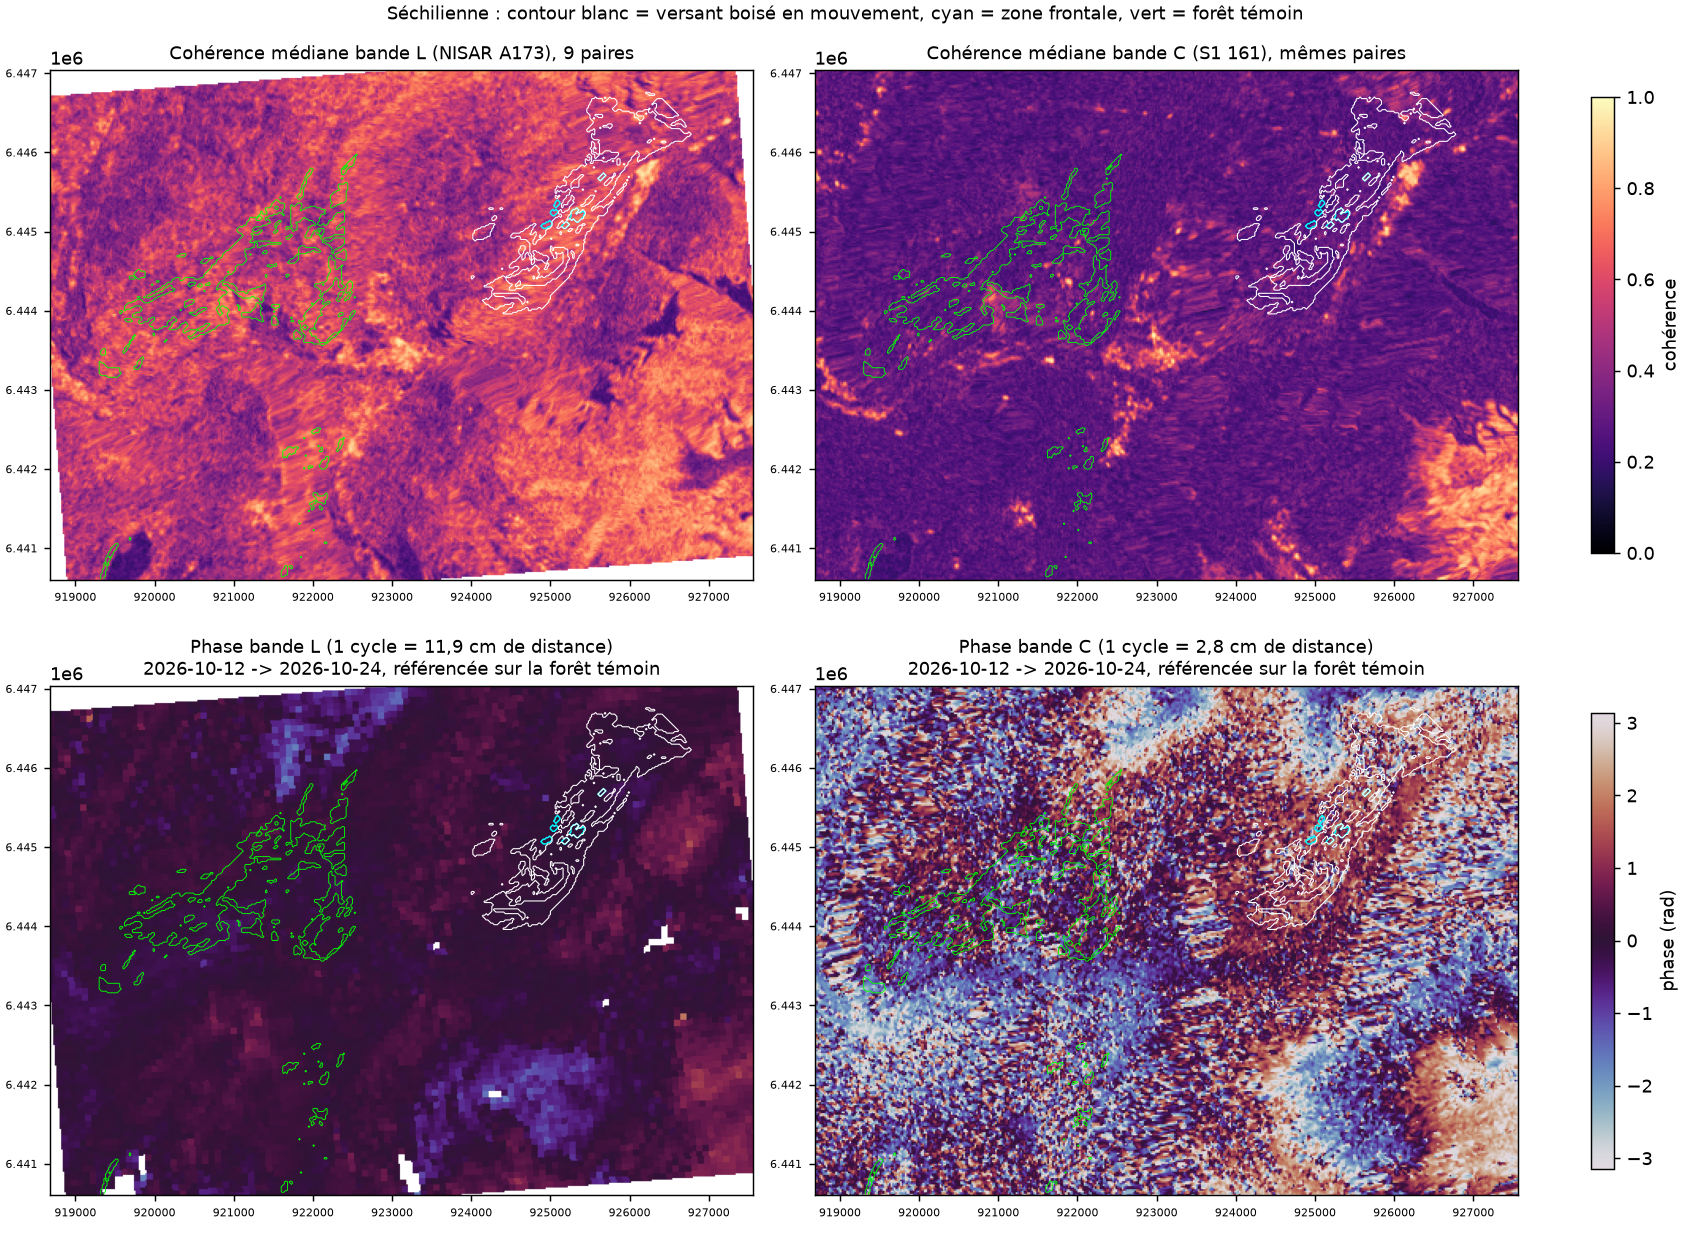
\includegraphics[width=0.66\linewidth, height=0.66\textheight, keepaspectratio]{g4_maps_A173.png}

	\scriptsize Versant boisé en mouvement (blanc), zone frontale (cyan), forêt témoin (vert) ; 17 paires
	appariées, 26/06 -- 24/10/2026.
\end{frame}

\begin{frame}{\phantom{x}}
	\frametitle{Glissement (2/2) : résultats}
	\vspace{-4pt}\scriptsize
	\centering
	\begin{tabular}{lcccc}
		\toprule
		Médiane sur les paires & \Lb{L A173} & \Cb{C A161} & \Lb{L D138} & \Cb{C D139}\\
		\midrule
		Cohérence, versant boisé & \textbf{0,58} & 0,28 & 0,32 & 0,29\\
		Consistance de phase, versant boisé & \textbf{0,92} & 0,11 & \textbf{0,88} & 0,09\\
		\bottomrule
	\end{tabular}

	\vspace{8pt}
	\raggedright
	\begin{itemize}
		\setlength{\itemsep}{2pt}
		\item \Cb{C} : décorrélée sous la forêt à 12~jours (0,97--0,99 sur le bâti : la chaîne est correcte)
		\item \Lb{L} : phase consistante à travers la canopée, condition nécessaire à l'InSAR de déplacement
		sous forêt
		\item Aucun déplacement au-dessus du bruit en 4 mois ($-4$ à $+5$~mm cumulés, bruit 3--10~mm par paire) :
		vitesse attendue de 1--5~cm/an trop faible pour des paires isolées
		\item Géométrie descendante défavorable : versant opposé à la visée
	\end{itemize}
\end{frame}

% ================================================================
\section{Synthèse}
% ================================================================

\begin{frame}{\phantom{x}}
	\frametitle{Synthèse : trois sites, un même message}
	\vspace{-4pt}\scriptsize
	\centering
	\begin{tabular}{p{2.3cm}p{3.6cm}p{3.4cm}p{3.6cm}}
		\toprule
		& \textbf{Vosges} (1 coupe) & \textbf{Morvan} (7 coupes) & \textbf{Séchilienne} (glissement)\\
		\midrule
		Forêt à 12~j & \Lb{0,64--0,70} / \Cb{0,28} & \Lb{0,35--0,71} / \Cb{0,25--0,36} & \Lb{0,58} / \Cb{0,28}\\
		Indicateur clé & AUC cohérence \Lb{0,995} / \Cb{0,74} & kappa du guide \Lb{0,41} / \Cb{0,08--0,16} &
		consistance de phase \Lb{0,92} / \Cb{0,11}\\
		Limite principale & n = 1 & 15~ha, IC larges & mouvement lent, 4 mois\\
		\bottomrule
	\end{tabular}

	\vspace{10pt}
	\begin{exampleblock}{À retenir}
		\scriptsize
		La \Lb{bande L} garde la forêt \textbf{cohérente} : une coupe y devient un \emph{événement}, et un versant
		boisé reste \emph{mesurable} en phase. La \Cb{bande C} reste utile en revisite et sur la strate basse :
		les deux sont complémentaires.
	\end{exampleblock}
\end{frame}

\begin{frame}{\phantom{x}}
	\frametitle{Regard critique et suite proposée pour le stage}
	\vspace{-6pt}\scriptsize
	\begin{columns}[T]
		\column{0.48\textwidth}
		\begin{alertblock}{Limites assumées}
			\scriptsize
			\begin{itemize}
				\setlength{\itemsep}{1pt}
				\item Petits échantillons, une saison par site
				\item Références optiques et photo-interprétées, sans terrain
				\item Estimateurs de cohérence différents (ISCE3 / SNAP) ; produits NISAR provisoires
				\item Bande P (BIOMASS) non testée : pas d'acquisition sur l'Europe de l'Ouest
			\end{itemize}
		\end{alertblock}
		\column{0.48\textwidth}
		\begin{block}{Ce que je propose de poursuivre}
			\scriptsize
			\begin{itemize}
				\setlength{\itemsep}{1pt}
				\item Détecteur combinant cohérence \Lb{L}, $\gamma^0$ \Lb{L} et revisite \Cb{C}, avec confirmation
				temporelle
				\item Plusieurs saisons et régions, dégâts de tempête
				\item Série NISAR $\geq$ 1 an et inversion SBAS (écosystème ISCE3) sur des glissements boisés,
				comparée aux mesures au sol
				\item Préparation de \textbf{ROSE-L} avec la même chaîne
			\end{itemize}
		\end{block}
	\end{columns}
\end{frame}

\begin{frame}
	\vfill
	\centering
	{\Large Merci pour votre attention !}

	\vspace{1em}
	\small\textcolor{mydgray}{Rapports complets (FR et EN), notes et code disponibles sur demande.}
	\vfill
\end{frame}

\begin{frame}[allowframebreaks]{Références}
	\scriptsize
	\nocite{torres2012sentinel1,snap,ose2015guide,drusch2012sentinel2}
	\printbibliography[heading=none]
\end{frame}

\end{document}
